\documentclass{article}
\usepackage[utf8]{inputenc}

\usepackage[OT2]{fontenc}
\usepackage[serbianc, serbian]{babel}
\usepackage{graphicx}


\usepackage{subfiles}
\usepackage{array}
\usepackage{float}

\title{Informacioni sistem za menad2ment transporta shec1era na podruchju Republike Srbije}
\author{Milica Gajic1, Marija Eric1, Milosh Kutleshic1}

\begin{document}

\maketitle
\newpage


\renewcommand*\contentsname{Sadrz1aj}
\tableofcontents
\newpage

\section{Uvod}
\subfile{uvod}
\section{Sluchajevi upotrebe}
\begin{figure}[h!]
    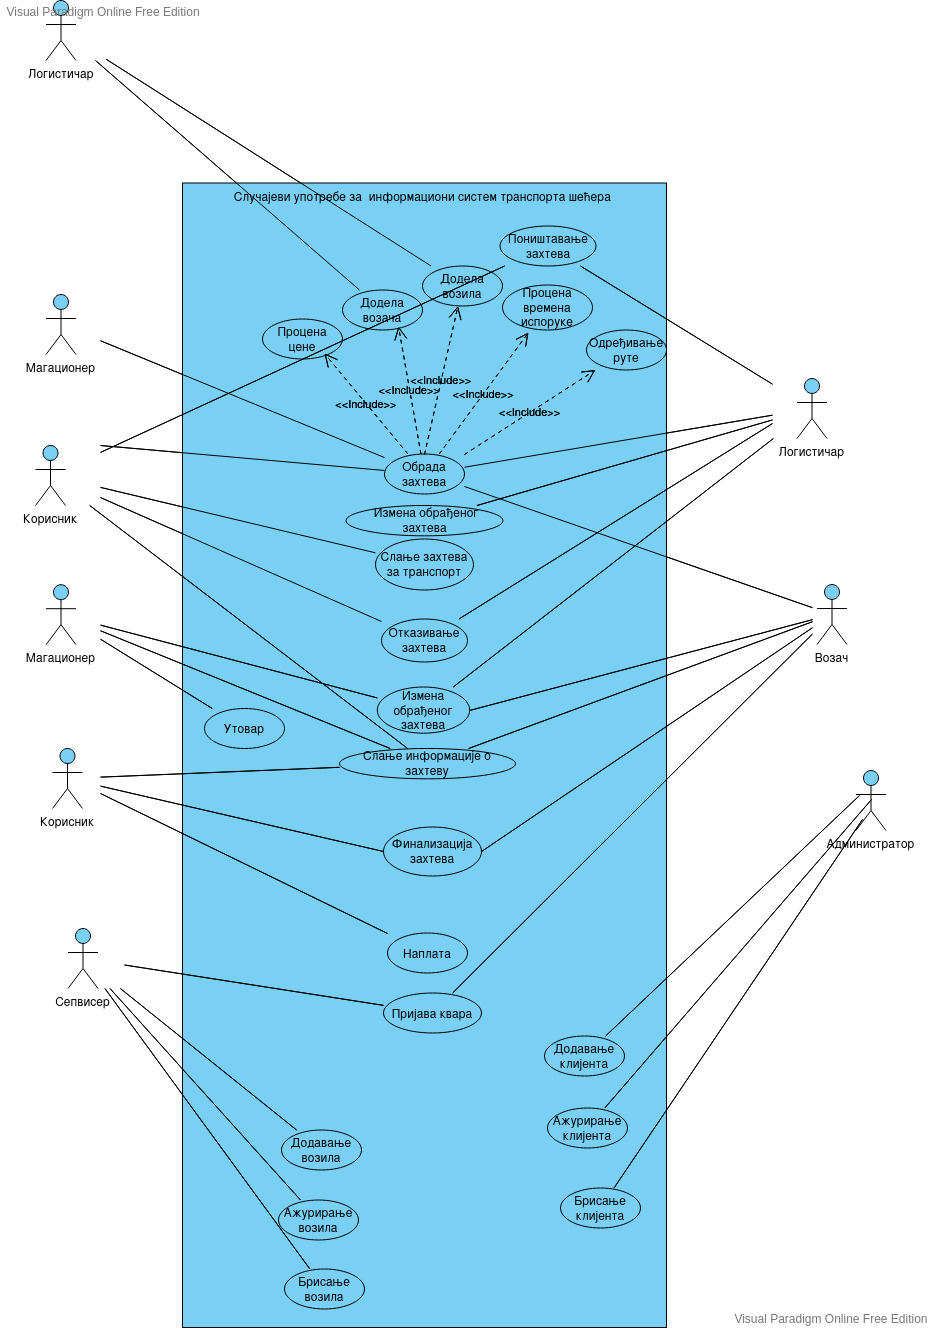
\includegraphics[scale = 0.2]{Slike/UML/SlucajeviUpotrebeSistema.jpg}
    \centering
    \caption{Sluchajevi upotrebe sistema za organizaciju transporta shec1era}
    \label{sistem}
\end{figure}  
U narednim sekcijama detaljno c1e biti obradjeni pojedinachni sluchajevi upotrebe sistema.

\subsection{Administrativni poslovi}

\subfile{SlucajeviUpotrebe/SUadministrativniPoslovi}

\subsection{Sluchaj upotrebe: Slanje zahteva za transport}
\subfile{SlucajeviUpotrebe/SUslanjeZahteva}

\subsection{Sluchaj upotrebe: Obrada zahteva za transport}
\subfile{SlucajeviUpotrebe/SUobradaZahteva}

\subsection{Sluchaj upotrebe: Izmena zahteva za transport}
\subfile{SlucajeviUpotrebe/SUizmenaZahteva.tex}

\subsection{Sluchaj upotrebe: Ponishtavanje zahteva za transport}
\subfile{SlucajeviUpotrebe/SUponistavanjeZahteva.tex}

\subsection{Sluchaj upotrebe: Dostavljanje porud2bine}
\subfile{SlucajeviUpotrebe/SUdostavljanjePorudzbine}
\subsection{Sluchaj upotrebe: Zavrshna faza proud2bine}
\subfile{SlucajeviUpotrebe/SUfinalizacijaPorudzbine}

\subsection{Odrzhavanje vozila}
\subfile{SlucajeviUpotrebe/SUodrzavanje}


\section{Model baze podataka sistema}
\subfile{ModelBaze}


\nocite{*}
\fontencoding{T1}\selectfont

\bibliography{literatura.bib}
\bibliographystyle{plain}


\end{document}
